\section{Problem Formulation}
\label{sec:formulation}
\subsection{Single Base Transceiver Station (BTS)}
Power consumed by a BTS, as a function of traffic load, can be
well approximated as a linear curve with a non-zero
y-intercept~\cite{Peng:2011:BTSSaving:Mobicom} given as
$P_1+l(P_2-P_1)/t_{max}$. Here $P_1$ and $P_2$ are the power
consumption at no load and full load, respectively, $l$ is the
number of calls presently being handled, and $t_{max}$ is the
maximum number of calls that can be handled.

Let $\delta$ be the traffic threshold at which the \textit{BTS
power savings} is applied (i.e., when BTS deactivates some TRXs
moving into low-power mode). If half of the TRXs are deactivated, $t_{max}$ drops by one half, too. At the same time, $P_2$ and $P_1$ also drop to by one half. The slope of the aforementioned linear power consumption profile for the BTS, therefore, is the same irrespective of the number of TRXs that are online. The power consumption profile wiht or without the BTS power-savings is shown in Figure~\ref{fig:powermodel1}. As
indicated in Figure~\ref{fig:powermodel1}, the no-load power
consumption drops to $P_1-\gamma$ in the low-power mode, where
$\gamma$ is a constant that depends on the equipment type and
the number of TRXs deactivated.

If $x$ is an indicator variable which is 1 when \textit{BTS
power savings} is applied, and $0$ otherwise, then the BTS
power consumption may be given by $P_1+l(P_2-P_1)/t_{max} -
(1-x)\gamma$, also indicated in Figure~\ref{fig:powermodel1} by
the piecewise linear solid line.

\begin{figure}
\centering
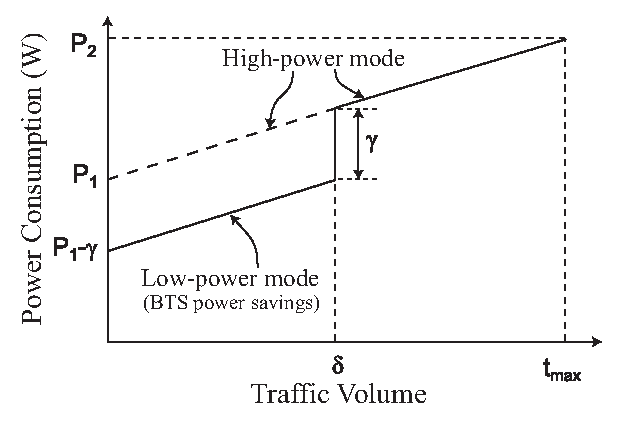
\includegraphics[width=0.46\textwidth]{figures/powermodel.eps}
\caption{BTS power consumption model. Low-power (BTS power savings) mode is optional and kicks in at low loads.}
\label{fig:powermodel1}
\end{figure}

The granularity of TRX deactivation can be increased to give the power consumption model in Figure~\ref{fig:powermodel2}. If the traffic is above threshold $\delta_2$, the BTS operates in the default high-power mode. When the traffic drops below threshold $\delta_2$, two TRXs are power-gated, and the BTS enter the medium-power mode (4+4+4 configuration). When the traffic falls below threshold $\delta_1$, two more TRXs are power-gated and the BTS enters the low-power mode. The drop in power consumption for each of the deactivation steps is $\gamma/2$, because compared to Figure~\ref{fig:powermodel1}, half as many TRXs are deactivated in each step.

\begin{figure}
\centering
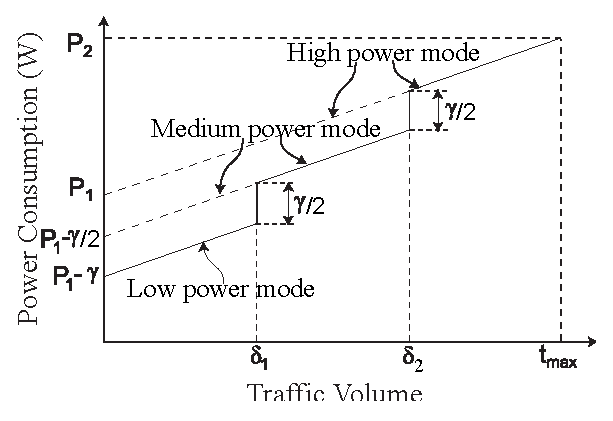
\includegraphics[width=0.46\textwidth]{figures/powermodel2-1.eps}
\caption{BTS power consumption model. BTS power saving is applied in a more granular way.}
\label{fig:powermodel2}
\end{figure}

The less granular model of Figure~\ref{fig:powermodel1} offers energy saving potential only when traffic falls to about one-third of the BTS capacity. The more granular model of Figure~\ref{fig:powermodel2}, on the other hand offers energy savings in two steps, with the first one kicking in as soon as the traffic falls below approximately two-third of the BTS traffic capacity. Therefore, the more granular model (Figure~\ref{fig:powermodel2}) should be more attractive for energy savings than the less granular one (Figure~\ref{fig:powermodel1}).

\subsection{Multi-BTS Cellular Setting}
Consider an area with $n$ active callers being served by $m$ BTSs.
We introduce indicator variable $w_{i,j}$, which is $1$ if call
$i$ \textit{is being} handled at BTS $j$ and $0$ otherwise. We
assume availability of an $n\times m$ matrix whose entry
$c_{i,j}$ is $1$ if caller $i$ \textit{can be} served through
BTS $j$ without exceeding the uplink or downlink budgets.
This information can be extracted by the data periodically
transmitted by each MS comprising the received signal strength
from nearby BTSs during a call. We also introduce indicator
variable $x_j$, which is $1$ if BTS $j$ is operating in
high-power mode (i.e., without \textit{BTS power savings}) and
$0$ otherwise. Using these variables and parameters, we can
formulate an optimization problem to minimize the total power
consumption over the network as:
\begin{align}
\textit{minimize} \quad \sum_{j=1}^{m} \left[
P_1+\sum_{i=1}^{n}\frac{w_{i,j}(P_2-P_1)}{t_{max}}-(1-x_j)\gamma
\right]
\end{align}
subject to the following constraints:
\begin{align}
& \sum_{j=1}^m w_{i,j} = 1 \qquad \forall i \\
& w_{i,j} \leq c_{i,j} \qquad \forall i, j \\
& \sum_{i=1}^nw_{i,j}-\delta \leq Mx_j \qquad \forall j%\\
\end{align}
\begin{align}
& \sum_{i=1}^n w_{i,j} \le t_{max} \qquad \forall i \\
%\end{align}
%\begin{align}
& w_{i,j}, x_j \in {0,1} \qquad \forall i, j%\\
%x_j \in {0,1}
\end{align}

We call this optimization problem, the two-step Low-Carb problem. The objective function is a simple generalization from the case
of one BTS. The first constraint ensures that no active call is
dropped just to save on power. The second constraint secures
the uplink budget by ensuring that no call is routed to a BTS
that can not handle it. The third constraint picks the correct
value for the decision variable $x_j$. The fourth constraint is the capacity constraint on all BTSs, while the last
constraint is the binary value constraint on the decision
variables.

For the three-step BTS power-saving model of Figure~\ref{fig:powermodel2}, the optimization problem can be stated as:
\begin{align}
\textit{minimize} \quad \sum_{j=1}^{m} \left[
P_1+\sum_{i=1}^{n}\frac{w_{i,j}(P_2-P_1)}{t_{max}}-\frac{(1-x_j)\gamma}{2}-\frac{(1-y_j)\gamma}{2}
\right]
\end{align}
subject to the following constraints:
\begin{align}
& \sum_{j=1}^m w_{i,j} = 1 \qquad \forall i \\
& w_{i,j} \leq c_{i,j} \qquad \forall i, j \\
& \sum_{i=1}^nw_{i,j}-\delta_1 \leq Mx_j \qquad \forall j\\
& \sum_{i=1}^nw_{i,j}-\delta_2 \leq My_j \qquad \forall j\\
%\end{align}
%\begin{align}
& \sum_{i=1}^n w_{i,j} \le t_{max} \qquad \forall i \\
%\end{align}
%\begin{align}
& w_{i,j}, x_j, y_j\in {0,1} \qquad \forall i, j%\\
%x_j \in {0,1}
\end{align}

In the above statement, we've added an indicator variable $y_j$, which is $1$ if BTS $j$ is in medium-power mode, $0$ otherwise. The fourth constraints ensures that $y_j$ takes on the proper value depending on the current traffic volume at BTS $j$. We call this optimization problem the three-step Low-Carb problem.


\subsection{Heuristic solutions to Low-Carb}
\label{subsec:heuristics} Both of the above optimization problems are Binary Integer Programs
(BIP), which is NP-Hard. It is intractable to solve it for an
operator's entire network, but solving it for a subset of the
network will provide some estimates of the amount of energy
savings possible using Low-Carb. Deployment to large operator
networks would require approximation algorithms. In this paper, we present two heuristics to solve the problem approximately and compare the results with the optimal solution.

\subsubsection{Heuristic 1}
\label{subsubsec:heuristic1} We describe here, the first heuristic for the two-step Low-Carb problem. Our first heuristic divides the set of BTSs $B$, into two disjoint subsets $B_1$ and $B_2$. Subset $B_1$ consists of those BTSs that have traffic above threshold $delta$. Subset $B_2$ consists of all other BTSs. Our heuristic shuffles the members of $B_1$ and iterates over the set. In every iteration, our heuristic looks at the current traffic load at a particular BTS. Let this traffic load be $h$. The heuristic declares that it must hand-off $h$-$delta$ calls away from the current BTS to it's neighbors in the subset $B_2$ while ensuring that no BTS in $B_2$ leaves it's subset as a result of the hand-off. This heuristic can be invoked multiple times, using a different shuffled order of BTSs in $B_2$ to improve the heuristic's performance. At the end of this process, members of $B_2$ are placed in low-power mode. 


For the three-step Low-Carb problem, members of $B_1$ are those BTSs that have traffic above threshold $delta_2$, while $B_2$ contains all other BTSs. We shuffle some calls from BTSs selected in a random order attempting to reduce the cardinality of set $B_1$. Once we are done iterating over all members of $B_1$, we re-initialize $B_1$ to contain BTSs that have traffic above threshold $delta_1$ and $B_2$ to contain all other BTSs and repeat the same call hand-off process as described earlier. In the end, those BTSs that have traffic above $\delta_1$ but below $\delta_2$ are placed in the medium-power mode while those with traffic below the $\delta_1$ threshold are palced in the low-power mode. Once again, this heuristic can be invoked multiple times to improve the probability of finding a near-optimal solution.

\subsubsection{Heuristic 2}
\label{subsubsec:heuristic2} We first describe the second heuristic for the two-step Low-Carb problem. In contrast to the first heuristic, the second one iterates over calls first. It first assigns all calls that only have one candidate BTS to the only BTS that can handle them.